\chapter{Validation of Application Energy Monitoring}
\label{chapter:validation}

\section{Introduction}

As described in \cref{chapter:implementation} we have implemented a proof-of-concept version of the Apollo Energy Allocator system, to prove the usefulness of our approach for allocating energy of underlying host systems to individual application requests running on them.  The software was tested during development to ensure correctness with respect to expected results through unit and integration tests, but now needs to be validated by using it in realistic test cases.  This process is described in this chapter.

In order to validate Apollo with realistic test cases, we need to define the kind of validation we are interested in achieving.  There are two main varieties of validation that we wish to achieve.

Firstly, we wish to validate the \emph{calculation correctness} of Apollo's results, by running the calculator in one or more controlled scenarios where we can also gather additional runtime statistics that allow a separate independent calculation of a fair energy consumption and manually perform these calculations and use them to check the correctness of Apollo's results in the same scenarios.

We also need to validate the \emph{consistency} of Apollo's results across a range of scenarios, to ensure that energy is allocated consistently with respect to the workload in the execution scenarios and host utilisation levels that prevail during them.

Another important area of validation is the \emph{allocation} of Apollo's results when a specific application scenario is run on a host machine with different amounts of competing workload.  As the competing workload rises, the energy allocation to the application scenario should fall, in proportion to its use of the machine.

Finally, an additional area of validation we wish to perform is to confirm that \emph{CPU is a valid proxy for overall resource usage} when performing energy allocation calculations.  For this validation we focus on how CPU usage varies for disk IO intensive workloads.

Throughout this validation testing we aim to achieve consistency of results to within 5\% tolerance.  Long experience teaches us that consistency is very difficult to achieve in any performance or resource utilisation testing due to the number of factors involved on a modern multi-cpu, multi-core server machine.  Our experience in previous testing work is that a 5\% tolerance in most cases is equivalent to equality plus the variation caused by factors outside our control.

\section{Testing Approach}

\subsection{The Test Application}
TODO - explain the microservice app

\subsection{The Test Software}
TODO - explain how tests were run and results captured including machine type, scripting, data capture and synthetic workload.

\section{Validating Calculation}

Our first point of validation is to ensure that the allocation calculation performed by Apollo can be reproduced by hand, following the algorithm presented in the previous chapter, with an acceptable level of consistency between the two approaches.

We chose one of the simpler standard scenarios that we had used during the testing process, the \texttt{simple-cpu-x50} scenario, which calls the CPU intensive service 50 times.  We decided to use a scenario based on just two services, the Gateway service and the CPU intensive service, both running on a single machine.  This was to keep the manual calculation process tractable and avoid inconsistencies and mistakes complicating the process.  The Apollo calculation algorithm is simply a process of aggregating results from individual application elements and so we were confident that if the result of calculation for a small number of application services was correct then this would result in a correct calculation process for more complex cases that were simply aggregations of the lower level calculations.

To perform the calculation process, we decided to use a different set of metrics data sources from the set used by Apollo, to validate the approach to data collection as well as the implementation of the algorithm.  The set of data that the calculations was based on was:


\begin{itemize}
	\item the \emph{Zipkin traces} from the scenario being studied, as there was no credible alternative to this data;
	\item the \emph{Docker network configuration} for the Docker subsystem that the application elements were running within, to allow the IP address to container mapping to be retrieved, and again this was the only source of this information;
	\item a set of \texttt{pidstat(1)} metrics for the application, showing the CPU utilisation every second for the application processes;
	\item a set of \texttt{mpstat(1)} metrics for the host machine which allowed us to assess how much CPU was being used by the host during the duration of the test trace;
	\item the \emph{SPECPower benchmark results} for a respresentative server model, similar to the host in use; and
	\item the output of the \texttt{ps(1)} command from the host machine with all of the application elements running, to allow the process IDs for the application elements to be retrieved.
\end{itemize}

The important point about the data sources we used for this calculation is that the key data sources for resource utilisation metrics were sourced from different mechanisms than those used by Apollo, to allow a broader degree of validation than a simple recalculation using identical data would have allowed.  While Apollo gets its resource utilisation metrics from the Docker subsystem's statistics mechanism (gathered via the Telegraf metrics server), for our calculations we used the metrics from mpstat(1) and pidstat(1) as explained above.

The first step was to inspect the Zipkin trace data to allow the start and end points of the request to be identified.  The Zipkin trace data had been saved from the execution of the test scenario and was loaded into a MySQL database to allow it to be queried easily.

The root traces were extracted from the Zipkin database, by selecting all of those rows in \texttt{zipkin\_spans} where the \texttt{trace\_id} column was the same as the \texttt{span\_id} column:

\lstset{language=SQL}
\begin{lstlisting}
select * from zipkin_spans where id=trace_id
\end{lstlisting}


From the row returned, we extracted a trace ID of \texttt{5896569591426873811}, a start time of \texttt{1534185668229000} (nano seconds since the "Epoch", equating to 20180813T184108.229Z), a duration of \texttt{126292740} (nano seconds - 126.292 seconds)	which imply an end time of \texttt{1534185794521740} (being equivalent to 20180813T184314.522Z).

Using the trace ID we could then run a more complex query to extract the trace's spans and their attributes from the Zipkin database:

\lstset{language=SQL}
\begin{lstlisting}
SELECT hex(s.trace_id) as trace_id, hex(s.id) as span_id,
       hex(s.parent_id) as parent_id,
       start_ts as start_time_usec, 
       start_ts+duration as end_time_usec,
       inet_ntoa(endpoint_ipv4 \& conv("ffffffff", 16, 10)) as ipv4_address,
       endpoint_port
FROM zipkin_spans s, zipkin_annotations a
WHERE s.trace_id = 5896569591426873811
AND s.trace_id = a.trace_id
AND s.id = a.span_id
AND a_key = 'sr'
ORDER BY start_ts
\end{lstlisting}

This allowed us to identify the spans making up the processing of the request and the IP addresses of the two application elements that handled the invocations as being \texttt{172.18.0.7} and \texttt{172.18.0.8}, which were the IP addresses of the Docker containers containing the microservices involved in handling the request.

The next step was a simple lookup of the IP addresses in the Docker network configuration which resulted in the container IDs of the two Docker containers that our application elements ran within.  The short form IDs returned were \texttt{c42b3d3bf4b2} for the Gateway container and \texttt{b75d29577eb9} for the CPU intensive container.

Having the container IDs allowed us to reliably identify the Linux process IDs of the Java virtual machines running our application elements.  By using the \texttt{ps} output we saved during the test execution, we could use the container IDs to find the Docker \texttt{docker-containerd-shim}  processes running the JVMs for our services, which were process 3278 for the CPU intensive service and 3436 for the Gateway service.

Having the process IDs allowed us to inspect the \texttt{pidstat} output that we had collected during the test execution.   This utility captured CPU percentage usage statistics for our processes every second during the test period.

For process 3278 (the CPU intensive service) we found that its average CPU consumption was 25.42\% with a very low standard deviation of 0.26 across the test set.

For process 3436 (the Gateway) we found that its average CPU consumption was 0.3\% of the machine (although this did have a maximum of 0.75\% for short periods, leading to a standard deviation of 0.11 for the test set).

We therefore decided to use 25.75\% as the container CPU usage during the test period.

The next step in the process was to estimate the energy usage of the underlying host machine.  We collected \texttt{sar} and \texttt{mpstat} resource utilisation metrics for the machine during the test period to provide host CPU utilisation metrics.  The \texttt{sar} statistics were of less use as this utility collects statistics every minute and so we had a limited number of samples, however it appeared to indicate a total machine CPU usage of about 25\% during the test period.

The \texttt{mpstat} statistics were more useful as they contained a metric measurement for CPU usage percentage per CPU every second during the test period.  When we analysed this data set we found that the machine's utilisation was a very constant 27\% right through the test period, apart from one second (10 seconds into the test) when it jumped to 75\% usage and then back down to 27\% (for reasons we weren't able to identify).

The CPU usage percentage allowed us to estimate the energy consumption of the machine using a representative set of SPEC Power benchmark results for a similar server model.  The benchmark results were 102W at 20\% and 120W at 30\%.  Therefore interpolation resulted in the value $((120 - 102) \times (7/10)) + 102 = 12.6 + 102 = 114.6$.  That is, the machine's power consumption during the test period was about 114 J/second.

Given that the test period was 126.30 seconds, this resulted in a power consumption value for the host machine of $126.30 \times 114 = 14473.98$J, which we rounded to 14474J.

Given the host CPU usage, the CPU usage of our containers and the host power consumption we could now calculate the power allocation to our application trace.

Given a test length of 126.3 seconds and a 4 CPU host machine this means a total possible CPU resource available of:

\begin{equation}
126.3 \times 4 = 505.2 ~\text{CPU seconds}
\end{equation}

Our test data indicates that the host was busy for 27\% of the time during the test execution, therefore our total host CPU time consumed during the test period was:

\begin{equation}
505.2 \times 0.27 = 136.40 ~\text{CPU seconds}
\end{equation}

Our application processes (containers) consumed 25.75\% of the host's CPU time during the test period therefore their CPU usage is calculated as:

\begin{equation}
136.40 \times 0.2575 = 130.09 ~\text{CPU seconds}
\end{equation}

Given our CPU usage and the host energy consumption we can then calculate the energy allocation to our application request as being:

\begin{equation}
130.09 / 136.40 \times 14474 = 13804\text{J}
\end{equation}

We then ran the Apollo proof of concept implementation on the test scenario data set to compare our results, which are shown in \tref{table:calculationresults}

\begin{table}
\centering
\caption{Manual Calculation Compared to Apollo Calculation}
\label{table:calculationresults}
\footnotesize
\begin{tabular}{|c|c|c|c|}
\hline
Value & Manual Calculation & Apollo Calculation & Difference \\
\hline
\hline
Trace CPU msec       & 130090 & 124257 & 4.5\% \\
Host CPU msec        & 136404 & 132891 & 2.5\% \\
Host Energy J        & 14474  & 14213  & 1.8\% \\
Application Energy J & 13804  & 13290  & 3.9\% \\
\hline
\end{tabular}
\end{table}

As can be seen from the results in the table, using a manual calculation technique that attempts to mirror the algorithm used in Apollo, while using different data sources for the critical resource utilisation metrics, has resulted in a very close match between the results, with the manual calculation of the energy allocation for the application request trace being within 4\% of the automated Apollo value.

The difference in the results will be familiar to anyone who has been involved in performance testing, where repeatability of results is often very difficult to obtain (as evidenced by the subtle but constant inconsistencies in the numerical results from tools such as \texttt{sar}, \texttt{mpstat} and \texttt{pidstat}).  In our situation, as well as the normal difficulty of repeatability, we believe that most of the difference in these results is likely to be the result of Apollo using the finer grained Docker metrics, while the manual process relied on the coarser grained metrics from the standard system administration tools. 

This result is well within our target tolerance for energy allocation results and so validates the Apollo proof of concept energy allocation implementation's accuracy.

\section{Validating Consistency}

To validate consistency of energy allocation, our strategy is to run a known control workload under fixed host utilisation conditions (no other workload being the simplest case) and to run a range of other workloads that we know contain an equivalent amount of computational work but are structured differently.  The energy allocation should be the same for each case.

In our first test, we structured a workload into three cases, each of which involved the same amount of CPU workload but in three different scenarios.  The first scenario invoked a short service call (involving 50msec of CPU work) 1000 times, the second scenario invoked a longer service call (500msec of CPU work) 100 times and the third ran a long service call (5000msec of CPU work) 10 times.  Each scenario was called 6 times to ensure a consistent result.

Our first question was whether the energy allocations per request were consistent across the three cases.  Our analysis of this question is shown in the scatter graph in \fref{figure:validation-energycpu}, which plots the energy usage against CPU workload for each of the scenarios executed, using logarithmic scales.

\begin{figure}
\centering
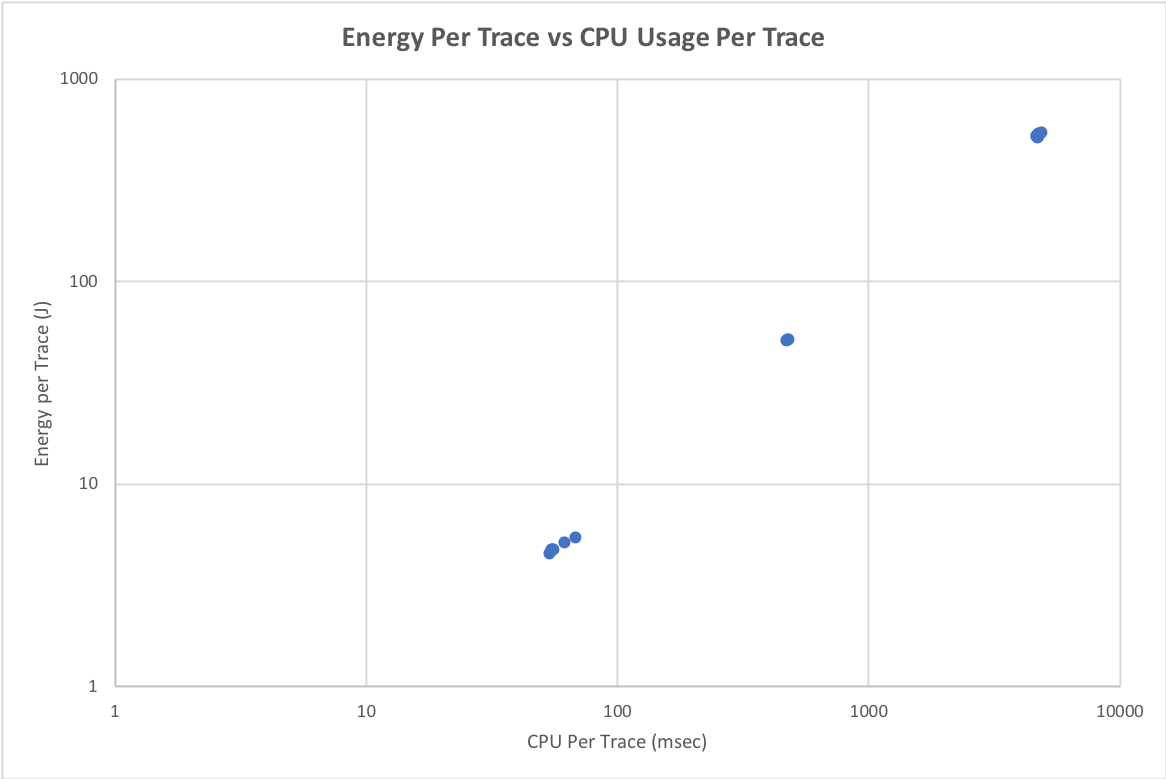
\includegraphics[width=1.0\textwidth]{Figures/validation-energycpu}
\caption{Energy Allocation per Request for Small, Medium and Large Services}
\label{figure:validation-energycpu}
\end{figure}

The graph shows the three sets of scenarios (short, medium and long) clearly clustering very closely, showing that the energy allocation per trace is extremely consistent across the three sets, suggesting that the allocation calculation is working consistently as designed.  More precisely, the correlation coeficient between the two sets of values is 0.999, indicating a very high degree of correlation between CPU consumed and energy allocation performed.

Our second test involved investigating how energy allocation was affected by a constant amount of CPU workload but in scenarios of different lengths.  To test this we ran repeatedly ran two scenarios, both of which contained the same amount of CPU workload (a trace that took 2,500 msec, run 50 times), with one scenario having pauses inserted into it, to cause the scenario to take longer to execute but consume no more CPU resource during the extended execution time.  In addition, for reasons which we explain below, we ran the first set of scenario tests with no additional load on the machine and the second set with synthetic workload consuming 50\% of the machine's CPU.  The results of this experiment are shown in the line graph in \fref{figure:validation-scenariolength}

\begin{figure}
\centering
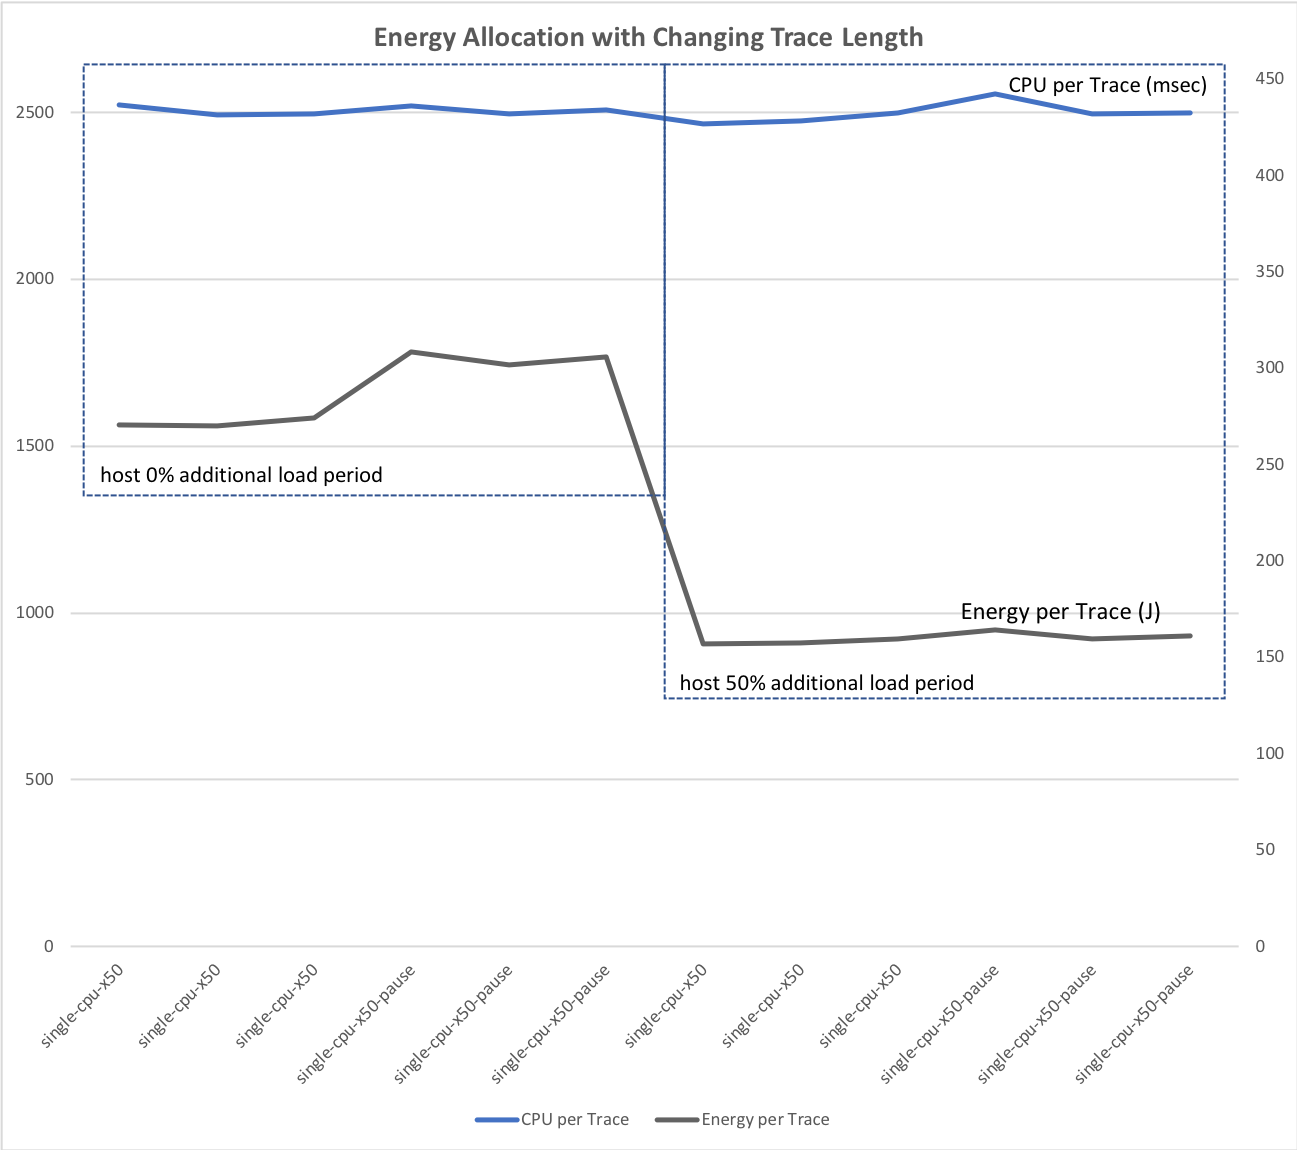
\includegraphics[width=1.0\textwidth]{Figures/validation-scenariolength}
\caption{Energy Allocation Across Different Scenario Lengths}
\label{figure:validation-scenariolength}
\end{figure}

This graph plots the CPU usage per trace (the top line) and the energy usage per trace (the bottom line) for sample executions of the scenarios.  As indicated by the dashed boxes annotating the graph, the first 6 executions were performed with no additional workload on the machine, the second 6 executions were performed with the machine having 50\% of its CPU capacity consumed by other synthetic workload.

As can be seen from the graph, the estimate of CPU usage by trace is consistent, within a maximum of 2\% variation from the mean (min 2467, max 2556, mean 2502, standard deviation of 23.09, which is less than 1\% of the mean).  This is well within our target consistency.

When we analysed the power allocation by trace we saw an interesting development which was the higher power allocation for the longer scenarios when no additional load was on the machine, an in constrast, a more constant power allocation when 50\% additional load was running on the machine.  While unintuitive initially, when we investigated the data, as explained below, we found that this is exactly as expected and is an important energy usage insight for the software architect investigating the power characteristics of their software in production.  

When no additional load is executing on the host, there is no other workload apart from our traces to allocate power consumption to.  In which case if the scenario takes longer, you would expect a higher energy allocation even with constant resource usage, as the host machine is consuming energy, even when not actively running our workload and if there is no other workload to allocate this "background" energy consumption to, then it will be allocated to our workload.  The graph shows that this is exactly what happens; when no other workload is executing on the machine, our longer scenarios (the "single-cpu-x50-pause" scenarios) are allocated more power than the shorter scenarios (the "single-cpu-x50" ones) even though they all consume very similar amounts of CPU time.

In contrast, when there is additional workload on the machine, the energy allocated to each trace is much more even, within a maximum of 4\% variation from the mean (min 157, max 164, mean 160, standard deviation of 2.66 which is 1.6\% of the mean).  This is also an expected result as during the execution of our test workload, there is other workload running on the machine which shares the allocation of the host's energy consumption.  As our workload runs longer, but is not using CPU during part of the period, it is allocated correspondingly less of the host's energy as there is other active workload on the machine which is allocated more of it.  This is the allocation we would expect and it is within our target consistency and again suggests that this is a consistent energy allocation mechanism.

\section{Validating Allocation}

Another aspect of energy allocation is how a fixed workload is allocated energy when the underlying host has varying amounts of other workload running on it concurrently.  We tested this aspect of allocation by running a single workload type under 5 different host utilisation conditions, namely when there was no other workload on the host, and when the host was 25\%, 50\%, 75\% and 100\% utilised before our workload started.  The results of this test are shown in the line graph in \fref{figure:validation-machineload}.

\begin{figure}
\centering
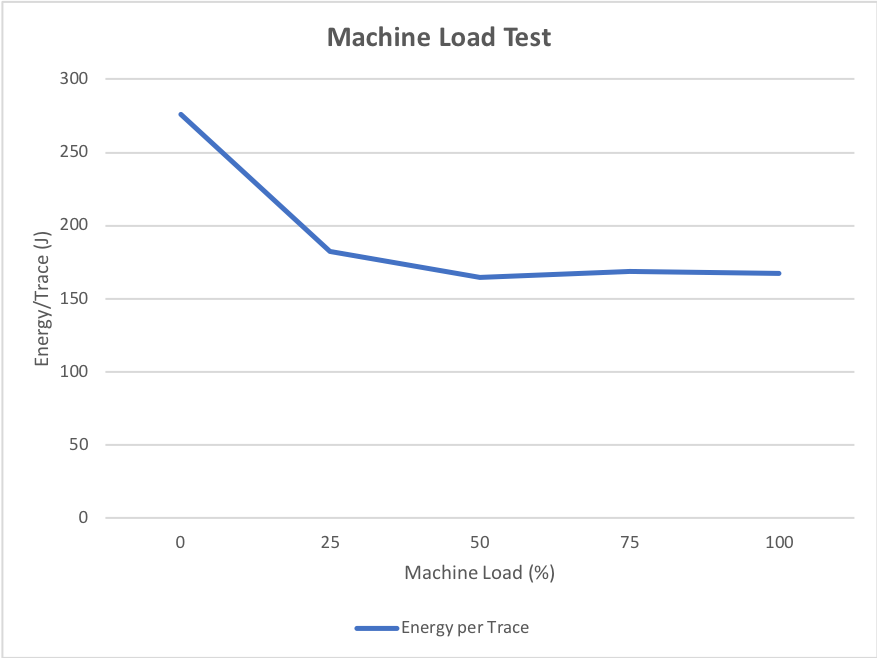
\includegraphics[width=1.0\textwidth]{Figures/validation-machineload}
\caption{Energy Allocation Under Different Host Load Conditions}
\label{figure:validation-machineload}
\end{figure}

As with some of our other testing, the results initially look somewhat counter intuitive, but on further analysis are validation of consistent energy allocation by workload.

%  (Trace J at 25/50/75/100 prior load: 276, 183 [93], 164 [19], 169, 167)

The first point in the graph shows our workload running on an otherwise idle host and it is allocated quite a large amount of energy per trace (of 276J) because the host is relatively inefficient at lower levels of utilisation and there is no other workload on the host to allocate its energy to.

The second point in the graph shows a sharp reduction in energy per trace (to 183J), which is caused by the host's utilisation now being about 50\% which is considerably more efficient than 25\% and the fact that the host's energy is being split between two roughly equivalent workloads.

The third point on the graph shows a further reduction in energy per trace (to 164J), which is a considerably smaller reduction than the previous step.  This is due to our share of the machine workload falling less significantly than in the previous step (from 49\% to 33\% whereas the previous step was from 96\% to 49\%).

The fourth point on the graph, at 75\% of other utilisation, actually goes up slightly (to 169J).  This is due to two factors.  Firstly, once again, our utilisation percentage drop decreases, this time from 33\% to 25\% (only 8\%) but secondly, the underlying machine becomes less efficient as utilisation moves beyond 75\% and so there is more energy to allocate between the different workload items.  This is an important insight for the application architect so that they consider the potentially non-linear energy consumption curve of the underlying host.

Finally at the fifth point on the graph, with 100\% other utilisation, our workload is competing with existing workload to be scheduled for execution.  This results in our execution duration extending slightly (by 5\%), and our CPU utilisation percentage to drop slightly (to 23\%) with the result being a slight reduction in energy utilisation (to 167J).  This is the result of a relatively small increase in the host's energy utilisation (as it was already running close to 100\% utilisation at the previous sample) and there is now further workload to allocate the energy of the host across, so reducing our workload's allocation slightly.

This phase of testing was an interesting process because it illustrated the usefulness of investigating energy allocation using practical testing and a quantitative data-based allocation mechanism like Apollo.  It would be quite possible to make a simplistic assumption that fair energy allocation would keep falling linearly as load increased, but our tool can be used to provide a more sophisticated analysis that reveals how a complex interaction of a number of factors (including load, scenario length and host energy characteristics) can result in a correct allocation that is more complex.  This is a useful insight for the application architect as they investigate the energy characteristics of their application.

\section{Validating CPU as a Resource Usage Proxy}

When we explained how the energy allocation process for an application's elements was to work, in \cref{chapter:monitoring}, part of the design of the allocation approach was to make the simplifying assumption that CPU utilisation is a good proxy for IO activity (\sref{sec:utilisingresourceusage}).  This allowed the the approach could ignore IO statistics and rely on CPU usage to allocate energy fairly.  While this assumption is based on previous research work, we were interested to test this assumption for ourselves by comparing IO activity with CPU utilisation.

To test the assumption that CPU utilisation acts as a good proxy for IO activity, we wanted to find whether the two values correlated well during an application workload.  To test this we ran IO intensive workloads of varying known sizes and measured the CPU utilisation of each one.  The results of this exercise are shown in the line graph in \fref{figure:validation-traceenergydatasize}.

\begin{figure}
\centering
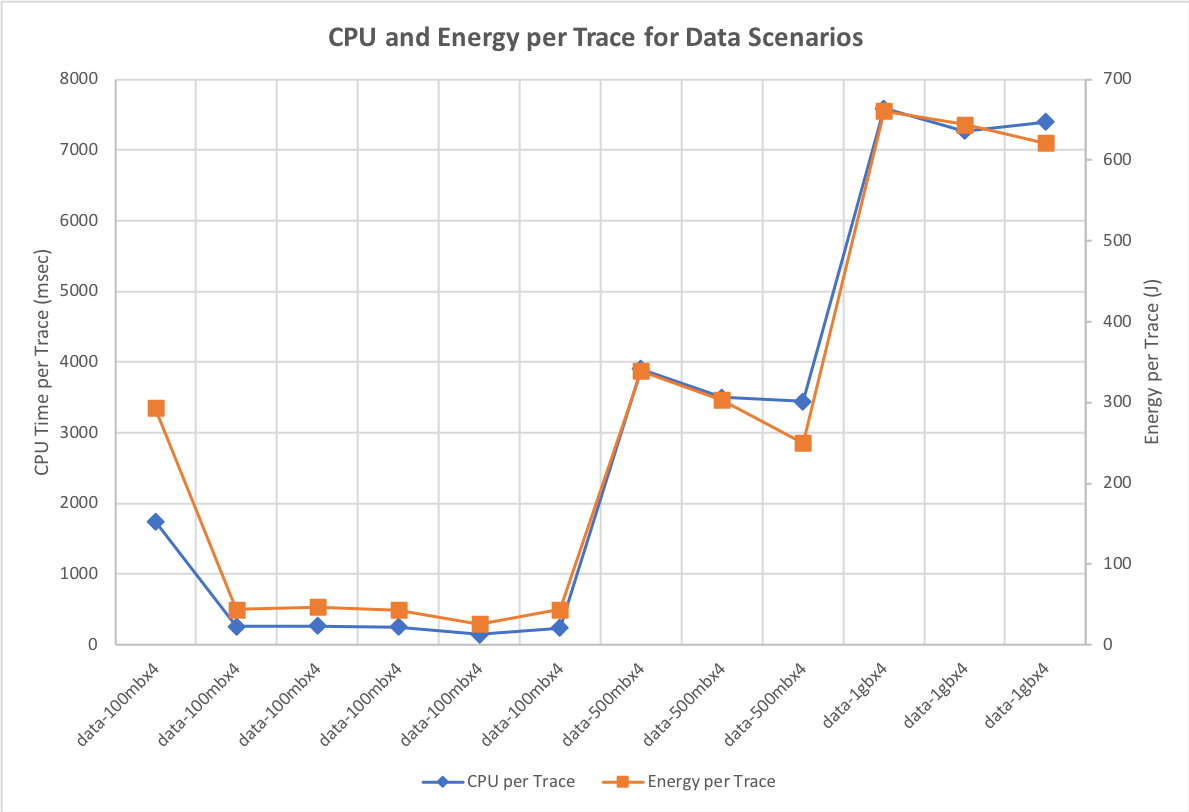
\includegraphics[width=1.0\textwidth]{Figures/validation-traceenergydatasize}
\caption{CPU Utilisation and Energy Allocation by Data Size}
\label{figure:validation-traceenergydatasize}
\end{figure}


sec:

\section{Summary}

